
\subsection{Analytical comparison of methods}

Both the direct method of section~\ref{sec:grad} and the EM algorithm of section~\ref{sec:EM_SSM}
have their strengths and weaknesses. Neither of them can be said to eclipse the other in an absolute sense.
In this section we will go through some features of the said algorithms found in the literature.
Then a more detailed analysis will be performed on two essential aspects of any estimation algorithm:
the convergence properties, i.e. when should one expect the algorithm to find a local maximum and
the computational requirements of the algorithms.

\textcite{Cappe2005} contains a list of arguments in favor of either of the methods. The following list includes
those and additional points with comments:
\begin{description}
  \item[Direct]\hfill
\begin{itemize}
  \item\emph{No smoother needed} The log-likelihood, or an approximation to it, can be evaluated
  with forward-filtering
  \item\emph{No M-step}. There is no need to figure out model-dependent maximization
  formulas even in nonlinear models 
  \item\emph{Faster convergence}. Advanced gradient-based optimization
  methods can reach convergence speeds that are close to quadratic
\end{itemize}
  \item[EM]\hfill
  \begin{itemize}
  \item \emph{Simple to implement}. This argument is often put forward in favor of the EM
 algorithm. However in practice when using the gradient-based method one would use any one of
the off-the-self nonlinear optimizers and not re-implement one. Thus which one is easier to implement
boils down to gradient computation. If the model is linear or linear-in-the-parameters the EM
algorithm doesn't need any gradient information.
  \item\emph{Parameter constraints}. In \textcite{Cappe2005} it is argued that
since the M-step maximization equations are so simple, including parameter constraints
are easier in the EM algorithm. This again depends on if the model is linear or linear-in-the-parameters.
  \item\emph{Parameterization independent}. This again depends on if one has to use gradient-based
 optimization in the M-step. If not, then the EM algorithm is parameterization independent. In the gradient-based
 method the gradient and the Hessian, and so the convergence, are affected by the parameterization.
\end{itemize} 
\end{description}


%%%%%%%%%%%%%%%%%%%%%%%%%%%%%%%%%%%%%%%%%%%%%%%%%%%%%%%%%
%%%% BALLISTIC OBJECT %%%%%%%%%%%%%%%%%%%%%%%%%%%%%%%%%%%
%%%%%%%%%%%%%%%%%%%%%%%%%%%%%%%%%%%%%%%%%%%%%%%%%%%%%%%%%

\subsection{Endoathmospheric flight of a ballistic projectile}\label{sec:ballistic}
Let us consider a situation where a ballistic projectile is launched
from the ground into the air. We assume that the situation is governed by Newtonian
mechanics and that the projectile experiences a constant known gravitational
force. In addition a velocity and altitude dependent drag force plays
a considerable role in the trajectory of the projectile \parencite{ristic2004beyond}. 
The drag force is caused by the air which might have a nonzero velocity with respect to the ground,
depending on the wind conditions.
 
We obtain a sequence of range measurements with a radar,
so that our data consists of the noisy two dimensional locations 
of the object as measured at time points $\brac{t_k}_{k=1}^T$.
We assume a constant interval $\tau$ between the time points.

Since the wind conditions are unknown, we supposet there is not
enough information for explicitly modeling the drag force. 
This is compensated by introducing
uncertainty into the dynamics with an additive stochastic process.
With these considerations, the system can be cast into a linear-Gaussian
SSM. 

% Newton's laws are specified in continous time,  where
% the dynamics can now be written as
% \begin{align}
% 	\dod{\x(t)}{t} &= \v{F}\x(t) + \gv{\beta}(t)
% 	\label{eq:ct_linear}
% \end{align}
% with
% \begin{align}
% 	\x(t) &= \bm{x(t) & \dot{x}(t) & \ddot{x}(t) & y(t) & \dot{y}(t) & \ddot{y}(t)}^\tr\\
% 	\v{F}&=\bm{
% 	&&1&&&\\
% 	&&&1&&\\
% 	&&&&1&\\
% 	&&&&&1\\
% 	&&&&&\\
% 	&&&&&\\
% 	}
% 	\label{tablelabel}
% \end{align}

To discretize the dynamics, we will apply a simple integration scheme where 
$\x(t)=\x(t_k)$ when $t\in\brak{t_k,t_{k+1}}$ \parencite{bar2004estimation}.
In this model, the state will contain the position and
its first and second time derivatives, i.e the velocity and the acceleration.
Without losing generality, we will write the model with unidimensional coordinates:
\begin{align}
	\x_k \equiv \x(t_k) &= \bm{x_k & \dot{x}_k & \ddot{x}_k }^\tr,
\end{align}
where
\begin{align}
	\x_k &= x(t_k)&\dot{x}_k &= \eval{\dod{x(t)}{t}}_{t=t_k}&\ddot{x}_k &= \eval{\dod[2]{x(t)}{t}}_{t=t_k}.
\end{align}
Then
\begin{align*}
	x_k &= \v{A}^{(1)}\xkk+\v{L}^{(1)}v_{k-1}&v_{k-1}\sim \N{0}{\sigma_x^2}\\
	y_k &=x_k+r_k & r_k \sim \N{0}{\sigma^2_r},
\end{align*}
where
\begin{align*}
	\v{A}^{(1)}&=\bm{
	1&\tau&\sfrac{\tau^2}{2}\\
	&1&\tau\\
	&&1
	}\\
	\v{L}^{(1)} &= \bm{
	\sfrac{\tau^2}{2} & \tau & 1\\
	}^\tr
\end{align*}
If we wish to replace $\v{L}^{(1)}v_{k-1}$ with the more familiar $\v{q}_{k-1}$,
then $\v{q}_{k-1}\sim \N{\v{0}}{\v{Q}^{(1)}}$ where
\begin{align}
	\v{Q}^{(1)} &= \sigma_x^2\v{L}^{(1)}(\v{L}^{(1)})^\tr = \sigma_x^2\bm{\frac{\tau^4}{4} & \frac{\tau^3}{2} &
	\frac{\tau^2}{2}\\
	\frac{\tau^3}{2} & \tau^2 & \tau\\ \frac{\tau^2}{2} & \tau & 1}
	\label{eq:ballistic_Q}
\end{align}
%
The generalization to $n$ dimensional coordinates includes $3\,n$
more states in $\x$ and it can be considered to consist of
$n$ independent systems with unidimensional coordinates.

We will simulate the situation in two dimensions and denote the components
of the resulting six dimensional state with
\begin{align}
	\xk &=
	\bm{x^{(1)}_k & \dot{x}^{(1)}_k & \ddot{x}^{(1)}_k 
	& x^{(2)}_k & \dot{x}^{(2)}_k & \ddot{x}^{(2)}_k }^\tr
	\label{eq:ballistic2D_state}
\end{align}
and the two dimensional measurements with
\begin{align}
	\yk &= \bm{y^{(1)}_{k} & y^{(2)}_{k} }^\tr.
	\label{eq:ballistic2D_measurementsl}
\end{align}
%
The model is then
\begin{align}
\begin{split}	
	\xk &=
	\bm{\v{A}^{(1)} & \\ & \v{A}^{(1)}}
	\xkk +\v{q}_{k-1}\\
	\yk &= \bm{1&0&0&0&0&0\\0&0&0&1&0&0}
	\xk+ \v{r}_k,
\end{split}
	\label{eq:ballistic2D_model}
\end{align}
where $\v{q}_{k-1}\sim \N{\v{0}}{\v{Q}}$ and $\v{r}_{k}\sim \N{\v{0}}{\v{R}}$
with
\begin{align}
	\v{Q} &= \bm{\sigma_1^2\v{L}^{(1)}(\v{L}^{(1)})^\tr & \\ & \sigma_2^2\v{L}^{(1)}(\v{L}^{(1)})^\tr}\\
	\v{R} &= \sigma_r^2\v{I}.
\end{align}
Additionally, the initial state $\x_0$ is assumed to be normally
distributed with $\N{\gv\mu_0}{\gv\Sigma_0}$, where
\begin{align}
	\gv\mu_0 &= \bm{0 & \cos(\alpha_0)v_0 & 0 & 
	0  & \sin(\alpha_0)v_0 & -9.81}^\tr\\
	\gv\Sigma_0 &= \mathrm{diag}\big(\bm{0 & 10^2 & 0 & 0 & 10^2 & 0}\big).
	\label{eq:ballistic_prior}
\end{align}
In other words, we assume the covariance matrix $\gv\Sigma_0$ diagonal and fully known
and specify further that the initial location and the initial acceleration
are deterministic and known. The mean of the initial velocity is parameterized
with $\alpha_0$ and $v_0$, which remain as parameters to be estimated.
%

Next we will focus on simulating measurements from the model and then estimating
the model parameters. The parameters of the initial distribution are chosen as
$\alpha_0 = \ang{50}$ and $v_0 = \SI{40}{m/s}$ and the initial state $\x_0$ is then
drawn from $\N{\gv\mu_0}{\gv\Sigma_0}$. The amount of drift in the gravitational force 
is controlled by the parameters $\sigma_1$ and $\sigma_2$.
These determine the standard deviations in the horizontal and vertical
components of the force per a single time step of duration $\tau$.
We will set 
\begin{align}
	\sigma_1&=\tau\,\si{m/s^2}\\
	\sigma_2&=\SI{0}{m/s^2}.
\end{align} 
%
Figure~\ref{fig:ballistic2D_simulation} presents  a simulated dataset, 
which is drawn from the two dimensional ballistic model with the aforementioned parameter
values.

Let us then proceed to maximum likelihood static parameter estimation. The training
data will be the simulated data, so that the true parameter values are the ones presented
earlier. In this case the most interesting parameter is probably the initial velocity,
i.e the angle $\alpha_0\in(0,\sfrac{\pi}{2})$ and the magnitude $v_0$, since it determines
the trajectory to a high degree.

 
Let us collect the parameters in the set $\Th=\brac{v_0,\alpha_0,\sigma_1,\sigma_2,\sigma_r}$.

 %
% To demonstrate filtering and smoothing, the filtering distributions were
% computed with the Kalman filter of section~\ref{sec:kalman_filter} and the smoothing distributions with
% the RTS smoother of section~\ref{sec:rts_smoother}. The results of the simulation are presented in
% Figure~\ref{fig:ballistic}. The uncertainty in the filtering distributions is noticeably larger
% when compared to the smoothing distributions, since the smoothing distributions
% include the information of the ``future'' measurements in addition to the past and the current ones.
% \todo{analyze the figure a bit more} 

\begin{figure}[htb]%
    \centering%
    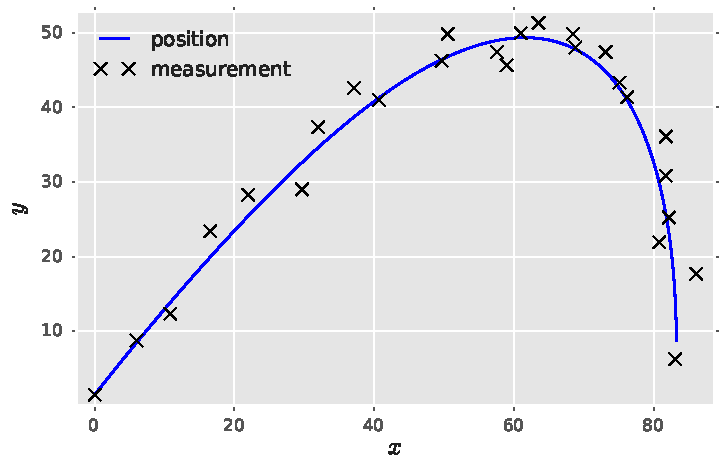
\includegraphics[width=0.6\textwidth]{img/ex1_pos_meas}%
	\caption{A simulation of the trajectory of a ballistic projectile with noisy measurements.}
	\label{fig:ballistic2D_simulation}
 \end{figure}
% \begin{figure}[htb]%
%     \centering%
%     \begin{subfigure}[b]{0.5\textwidth}%
%     	\centering%
%     	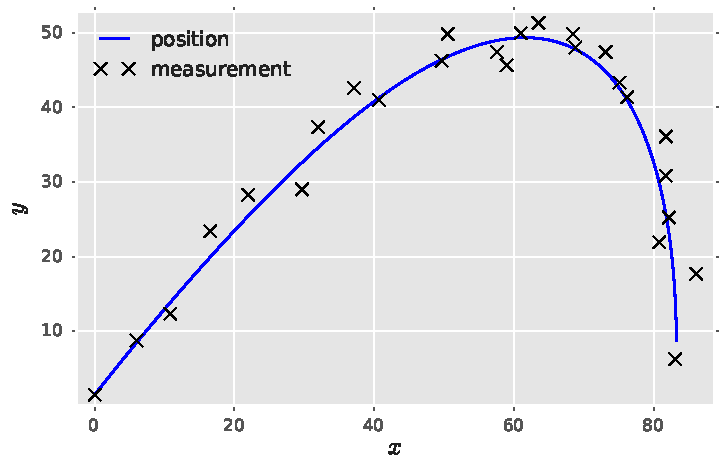
\includegraphics[width=\textwidth]{img/ex1_pos_meas}%
%     	%\missingfigure{Plot}
%     	\caption{The noisy measurements are plotted with crosses. The initial point is at the origo.}%
% 		\label{fig:ballistic_flight}%
%     \end{subfigure}%
%     \begin{subfigure}[b]{0.5\textwidth}%
%     	\centering%
% 		\includegraphics[width=\textwidth]{img/ex1_err}%
%     	%\missingfigure{Plot}
%     	\caption{Error mean with $\pm 2$ standard deviations in $\dot{x}$ for the filter and the smoother}%
% 		\label{fig:ballistic_err}%
%     \end{subfigure}%
% 	\caption{A simulation of the the ballistic object in 
% 	Example~\ref{ex:ballistic}.}
% 	\label{fig:ballistic}
%  \end{figure}


\missingfigure{Error as a function of iterations for $100$ independent simulations for BFGS}
\missingfigure{Error as a function of iterations for $100$ independent simulations for EM}

\parencite{ristic2004beyond,Ratna2008,Lindsten2010}

%%%%%%%%%%%%%%%%%%%%%%%%%%%%%%%%%%%%%%%%%%%%%%%%%%%%%%%%%%%%%%%%
%%%%%%%%%%%%%%%%%%%% HEART %%%%%%%%%%%%%%%%%%%%%%%%%%%%%%%%%%%%%
%%%%%%%%%%%%%%%%%%%%%%%%%%%%%%%%%%%%%%%%%%%%%%%%%%%%%%%%%%%%%%%%

\subsection{Decomposing an electrocardiograph with frequency tracking}
\missingfigure{Error as a function of iterations for $100$ independent simulations for BFGS}
\missingfigure{Error as a function of iterations for $100$ independent simulations for EM}
\parencite{Sarkka2012}
